\subsection{Hàm đa biến}
\begin{frame}
\frametitle{Hàm đa biến}
\begin{figure}
    \centering
    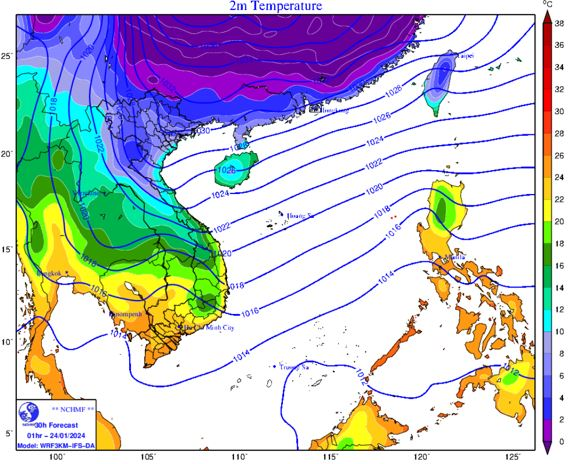
\includegraphics[width=0.5\textwidth]{Content/Figure/TemperatureGraph.jpg}
    \caption{Biểu đồ nhiệt độ theo khu vực}
\end{figure}
\end{frame}

\begin{frame}
\frametitle{Hàm đa biến}
\begin{tcolorbox}[colback=blue!10!, colframe=blue!50!black, title=Định nghĩa]
    Hàm \(f\) theo \(n\) biến là quy tắc gán một véc-tơ \( \mathbf{x} = (x_1, x_2, \ldots, x_n) \) trong tập xác định \(D \subseteq \mathbb{R}^n\) với một số thực \(f(\mathbf{x})\).
\end{tcolorbox}
\begin{figure}
    \centering
    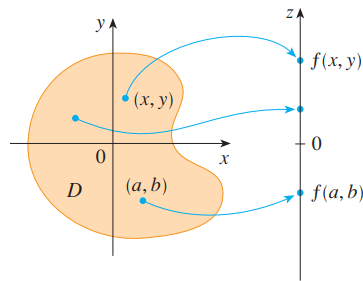
\includegraphics[width=0.3\textwidth]{Content/Figure/MultiVariable.png}
    \caption{Hàm số hai biến \(z = f(x, y)\)}
\end{figure}
\end{frame}

\begin{frame}
\frametitle{Hàm đa biến}
\begin{columns}
\column{0.5\textwidth}
Đồ thị hàm \(f\) bao gồm mọi điểm \((x_1, x_2, \ldots, x_n, z)\) trong \(\mathbb{R}^{n+1}\) sao cho \(z = f(x_1, x_2, \ldots, x_n)\).
\begin{figure}
    \centering
    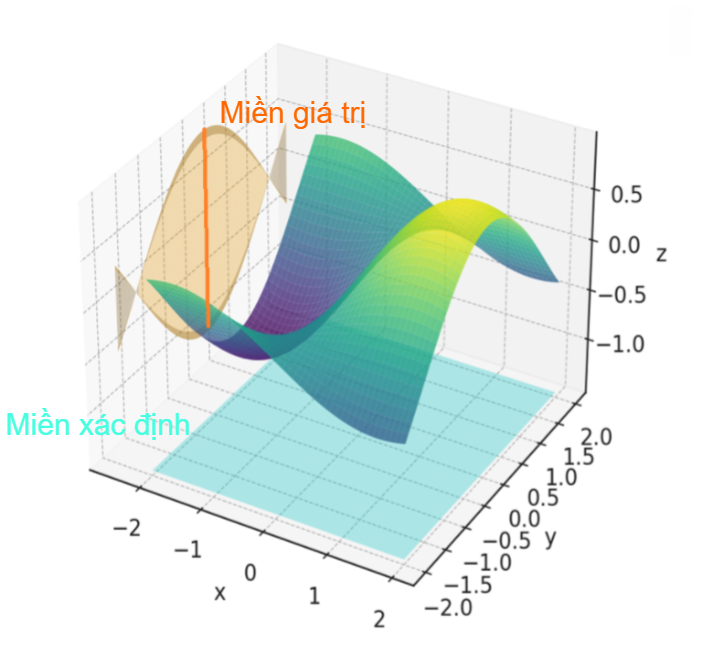
\includegraphics[width=0.65\textwidth]{Content/Figure/Domains.png}
    \caption{Miền giá trị và miền xác định}
\end{figure}
\column{0.5\textwidth}
Một số ví dụ:
\begin{itemize}
    \item \(z=\sin x + \cos y\): \(D = \mathbb{R}^2\), \(z \in [-2, 2]\)
    \item \(z=\sqrt{x+y+1}\): \(D = \{(x,y) | x+y+1 \geq 0\}\), \(z \in [0, +\infty)\)
\end{itemize}
\begin{figure}
\centering
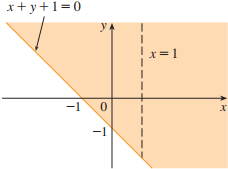
\includegraphics[width=0.5\textwidth]{Content/Figure/MienXacDinh.png}
\caption{Miền xác định của hàm \(z=\sqrt{x+y+1}\)}
\end{figure}
\end{columns}
\end{frame}

\begin{frame}
\frametitle{Hàm đa biến}
Đồ thị đường mức của hàm \(f(\mathbf x)\) là tập hợp véc-tơ \(\mathbf x\) sao cho \(f(\mathbf x)=c\) với một hằng số \(c\).
\begin{columns}
\column{0.5\textwidth}
\begin{figure}
    \centering
    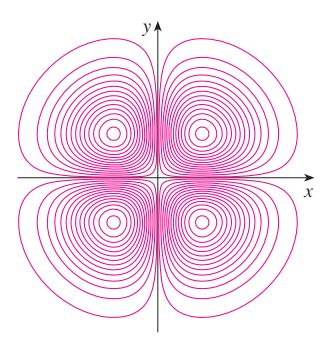
\includegraphics[width=0.53\textwidth]{Content/Figure/contour2d.png}
    \caption{Đường mức của hàm \(z=xy e^{-(x^2+y^2)}\).}
\end{figure}
\column{0.5\textwidth}
\begin{figure}
    \centering
    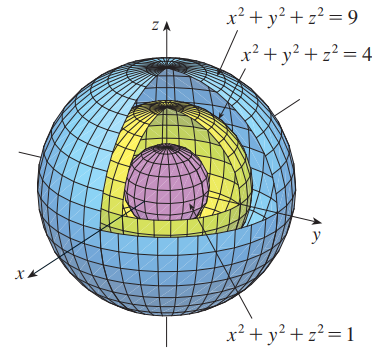
\includegraphics[width=0.61\textwidth]{Content/Figure/contour3d.png}
    \caption{Đường mức của hàm \(f=x^2+y^2+z^2\)}
\end{figure}
\end{columns}
\end{frame}

\subsection{Đạo hàm riêng}
\begin{frame}
\frametitle{Đạo hàm riêng}
\begin{tcolorbox}[colback=blue!10!, colframe=blue!50!black, title=Định nghĩa]
Đạo hàm riêng của hàm \(f(\mathbf x)\) theo \(x_i\) tại điểm \(\mathbf{a} = (a_1, a_2, \ldots, a_n)\) là giới hạn
\begin{equation}
f_{x_i}=\frac{\partial f}{\partial x_i}(\mathbf{a}) = \lim_{h \to 0} \frac{f(a_1, \ldots, a_{i-1}, a_i + h, a_{i+1}, \ldots, a_n) - f(a_1, a_2, \ldots, a_n)}{h}
\end{equation}
nếu giới hạn này tồn tại.
\end{tcolorbox}
Khi này, vi phân của hàm \(f\) tại điểm \(\mathbf{a}\) có thể được biểu diễn như sau:
\begin{equation}
df = f_{x_1} dx_1 + f_{x_2} dx_2 + \ldots + f_{x_n} dx_n
\end{equation}
\end{frame}

\begin{frame}
\frametitle{Đạo hàm riêng}
Xét đồ thị hàm số \(z(x, y)\). Mặt phẳng \(x=a\) và \(y=b\) cắt đồ thị tại hai đường cong \(C_2\) và \(C_1\). Khi đó các đạo hàm riêng chính là độ dốc của các tiếp tuyến \(T_2\) và \(T_1\) của hai đường cong tại điểm \(P(a, b, c)\).
\begin{figure}
    \centering
    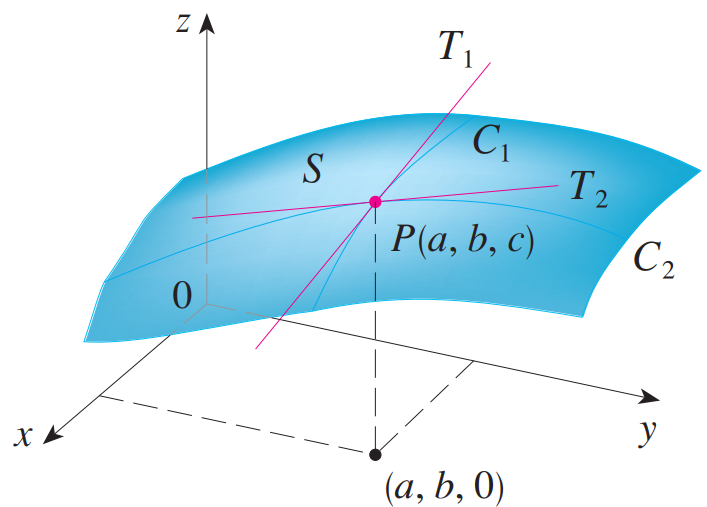
\includegraphics[width=0.4\textwidth]{Content/Figure/PartialDerivatives.png}
    \caption{Ý nghĩa hình học của đạo hàm riêng}
\end{figure}
\end{frame}

\begin{frame}
\frametitle{Đạo hàm riêng}
\begin{tcolorbox}[colback=blue!10!, colframe=blue!50!black, title=Định lý Clairut]
Nếu hàm \(f(x,y)\) có đạo hàm riêng bậc nhất liên tục lân cận điểm \((a,b)\) thì
\begin{equation}
f_{xy}(a,b) = f_{yx}(a,b)
\end{equation}
\end{tcolorbox}
\small
Định lý trên thường được sử dụng trong nhiệt động lực học. Ví dụ, ta có các hàm \(F(T, V)\), \(P(T, V)\), \(S(T, V)\) có các vi phân liên hệ với nhau: \(dF=-SdT-PdV\).

Áp dụng định lý Clairut:
\begin{equation}
F_{TV} = F_{VT} \Rightarrow \left(\frac{\partial S}{\partial V}\right)_T = \left(\frac{\partial P}{\partial T}\right)_V
\end{equation}
Phương trình trên là một trong các phương trình Maxwell trong nhiệt động lực học.
\normalsize
\end{frame}

\subsection{Gradient}
\begin{frame}
\frametitle{Gradient}
\begin{tcolorbox} [colback=blue!10!, colframe=blue!50!black, title=Định nghĩa]
    \textbf{Trường vô hướng} gán tương ứng một giá trị vô hướng cho mọi điểm trong không gian.
\end{tcolorbox}
Ví dụ:
\begin{itemize}
\item Trong bản đồ nhiệt độ, nhiệt độ \(T(\varphi, \lambda)\) được gán với các kinh độ và vĩ độ.
\item Trong trường điện từ, điện thế \(V(x, y, z)\) được gán với các tọa độ trong không gian.
\end{itemize}
\end{frame}

\begin{frame}
\frametitle{Gradient}
\begin{tcolorbox} [colback=blue!10!, colframe=blue!50!black, title=Định nghĩa]
    \textbf{Gradient} của trường vô hướng \(f(x, y, z)\) là véc-tơ
    \begin{equation}
    \nabla f = f_x \mathbf{\hat{x}}+f_y \mathbf{\hat{y}} + f_z \mathbf{\hat{z}}
    \end{equation}
\end{tcolorbox}
Như vậy, ta có thể viết tìm biến thiên \(df\) của hàm \(f\) khi dịch chuyển một đoạn \(d\mathbf r=(dx, dy, dz)\) trong không gian như sau:
\begin{equation}
df = f_x dx + f_y dy + f_z dz = \nabla f \cdot d\mathbf r
\end{equation}
\end{frame}

\begin{frame}
\frametitle{Gradient}
Về mặt hình học, gradient \(\nabla f\) chỉ hướng tăng nhanh nhất của hàm \(f\) và có độ lớn bằng độ dốc theo hướng này.
\begin{figure}
    \centering
    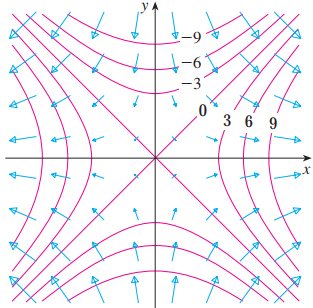
\includegraphics[width=0.3\textwidth]{Content/Figure/gradient.png}
    \caption{Ý nghĩa hình học của gradient}
\end{figure}
\end{frame}

\subsection{Tích phân đa biến}
\begin{frame}
\frametitle{Tích phân bội}
Làm thế nào để tính thể tích của một paraboloid \(z=x^2+y^2\) nằm dưới mặt phẳng \(z=a\)?
\begin{figure}
    \centering
    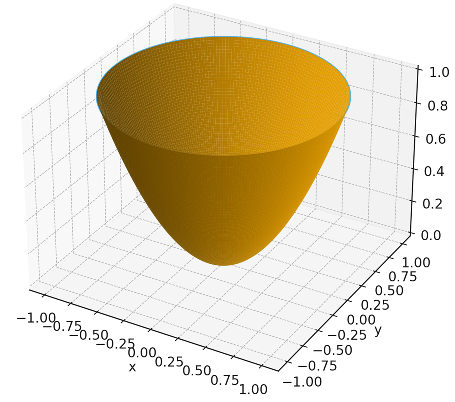
\includegraphics[width=0.4\textwidth]{Content/Figure/paraboloid.png}
    \caption{Paraboloid}
\end{figure}
\end{frame}

\begin{frame}
\frametitle{Tích phân bội}
\begin{columns}
    \column{0.5\textwidth}
    Thể tích \(V\) của paraboloid có thể được tính bằng tổng thể tích của các đĩa dày \(dz\):
    \begin{figure}
        \centering
        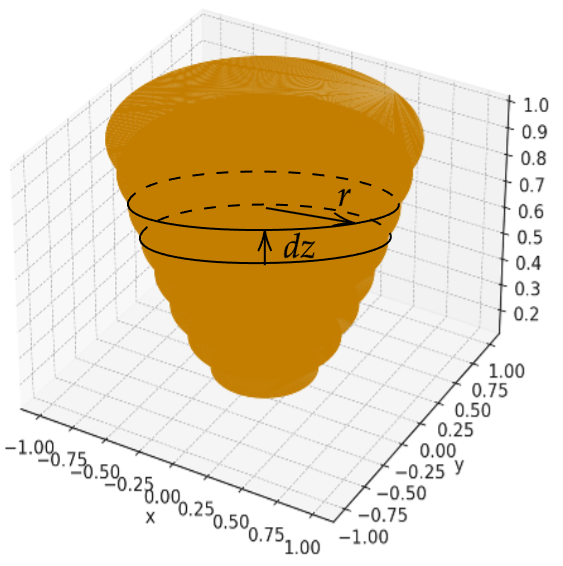
\includegraphics[width=0.7\textwidth]{Content/Figure/discs.png}
    \end{figure}
    \column{0.5\textwidth}
    Trong hệ tọa độ trụ, diện tích của mỗi đĩa được tính bằng tổng diện tích các tam giác nhỏ có góc nhọn \(d\phi\):
    \begin{figure}
        \centering
        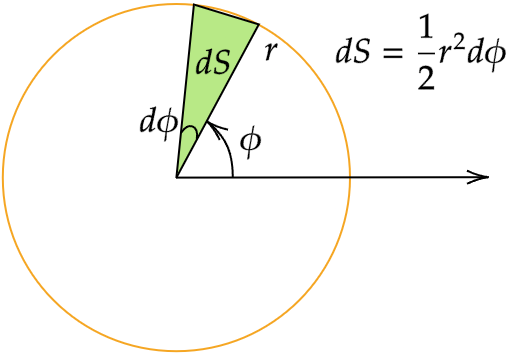
\includegraphics[width=0.8\textwidth]{Content/Figure/cylindricaldisc.png}
    \end{figure}
\end{columns}
\end{frame}

\begin{frame}
\frametitle{Tích phân bội}
Khi đó, thể tích \(V\) có thể được tính như sau:
\begin{equation}
    V= \int_0^a \int_0^{2\pi} \dfrac{r^2}{2} d\phi dz
\end{equation}
Biểu thức trên là một \textbf{tích phân hai lớp}.

Như vậy, thể tích của paraboloid là:
\begin{equation}
    \begin{aligned}
    V&= \int_0^a \pi r^2 dz\\
    &= \int_0^a \pi z dz = \boxed{\dfrac{\pi a^2}{2}}
    \end{aligned}
\end{equation}
\end{frame}

\begin{frame}
\frametitle{Tích phân bội}
\begin{columns}
\column{0.5\textwidth}
Trong hệ tọa độ Đề-các, diện tích của đĩa được tính bằng tổng diện tích của các hình vuông nhỏ có chiều rộng \(dy\):
\begin{figure}
    \centering
    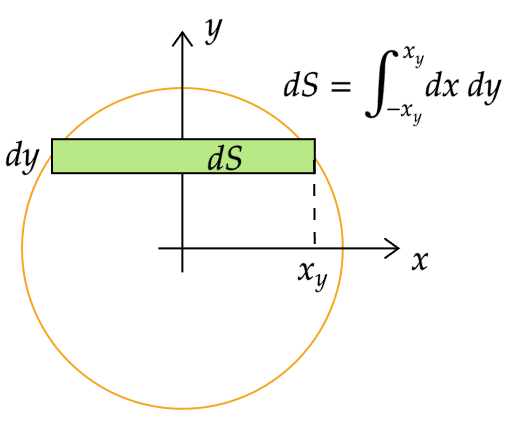
\includegraphics[width=0.7\textwidth]{Content/Figure/descartesdisc.png}
\end{figure}
\column{0.5\textwidth}
Khi đó, thể tích \(V\) có thể được tính như sau:
\begin{equation}
    V= \int_0^a \int_{-\sqrt{z}}^{\sqrt{z}} \int_{-\sqrt{z-y^2}}^{\sqrt{z-y^2}} dx dy dz
\end{equation}
Biểu thức trên là một \textbf{tích phân ba lớp}.

Thực hiện phép tích phân trên, cuối cùng ta vẫn thu được:
\begin{equation}
    V = \boxed{\dfrac{\pi a^2}{2}}
\end{equation}
\end{columns}
\end{frame}

\begin{frame}
\frametitle{Tích phân đường}
Gọi \(\mathbf v(x, y, z)\) là một hàm véc-tơ ứng với mọi điểm trong không gian. \(C\) là một đường cong trong không gian nối hai điểm \(\mathbf a\) và \(\mathbf b\), và có véc-tơ chỉ phương là \(\mathbf u\).
\begin{figure}
    \centering
    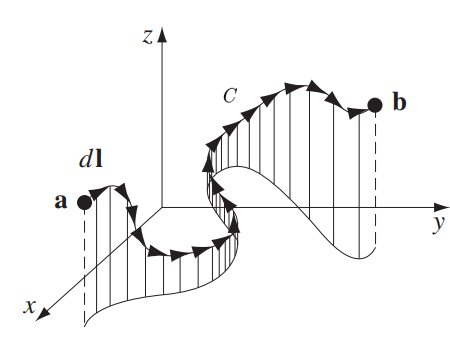
\includegraphics[width=0.3\textwidth]{Content/Figure/tichphanduong.png}
\end{figure}
Khi đó tích phân đường của \(\mathbf v\) dọc theo \(C\) là:
\begin{equation}
\int_C \mathbf v \cdot \mathbf u dl= \int_C \mathbf v \cdot d\mathbf l.
\end{equation}
\end{frame}

\begin{frame}
\frametitle{Tích phân đường}
\begin{tcolorbox}
[colback=blue!10!, colframe=blue!50!black, title=Định lý cơ bản của giải tích]
Nếu \(f\) là một hàm vô hướng có đạo hàm liên tục trong miền chứa đường cong \(C\) nối hai điểm \(\mathbf a\) và \(\mathbf b\), thì
\begin{equation}
\int_C \nabla f \cdot d\mathbf l = f(\mathbf b) - f(\mathbf a).
\end{equation}
\end{tcolorbox}
\end{frame}

